\documentclass[12pt, letterpaper]{article}
\usepackage[titletoc,title]{appendix}
\usepackage{color}
\usepackage{booktabs}
\usepackage[usenames,dvipsnames,svgnames,table]{xcolor}
\definecolor{dark-red}{rgb}{0.75,0.10,0.10} 
\usepackage[margin=1in]{geometry}
\usepackage[linkcolor=dark-red,
            colorlinks=true,
            urlcolor=blue,
            pdfstartview={XYZ null null 1.00},
            pdfpagemode=UseNone,
            citecolor={dark-red},
            pdftitle={Typecast: A Routine Mental Shortcut Causes Party Stereotyping}]{hyperref}

\usepackage[resetlabels,labeled]{multibib}
\newcites{SI}{SI References}
\usepackage{natbib}
\usepackage[section]{placeins}
\usepackage{float}

\usepackage{geometry} % see geometry.pdf on how to lay out the page. There's lots.
\geometry{letterpaper}               % This is 8.5x11 paper. Options are a4paper or a5paper or other... 
\usepackage{graphicx}                % Handles inclusion of major graphics formats and allows use of 
\usepackage{amsfonts,amssymb,amsbsy}
\usepackage{amsxtra}
\usepackage{verbatim}
\setcitestyle{round,semicolon,aysep={},yysep={;}}
\usepackage{setspace}             % Permits line spacing control. Options are \doublespacing, \onehalfspace
\usepackage{sectsty}             % Permits control of section header styles
\usepackage{lscape}
\usepackage{fancyhdr}             % Permits header customization. See header section below.
\usepackage{url}                     % Correctly formats URLs with the \url{} tag
\usepackage{fullpage}        %1-inch margins
\usepackage{multirow}
\usepackage{rotating}
\usepackage{comment}
\setlength{\parindent}{3em}

\usepackage[T1]{fontenc}
%\usepackage{bm}
\usepackage{libertine}

\usepackage{chngcntr}

%This section double-spaces & makes footnotes the same size as normal text.
%\usepackage{footmisc}
%\setlength{\footnotesep}{\baselineskip}
%\makeatother
%\renewcommand{\footnotelayout}{\normalsize \doublespacing}

% Alternative citation styles
\def\citeapos#1{\citeauthor{#1}'s (\citeyear{#1})}


% Caption
\usepackage[hang, font=small,skip=0pt, labelfont={bf}]{caption}
%\captionsetup[subtable]{font=small,skip=0pt}
\usepackage{subcaption}

% tt font issues
% \renewcommand*{\ttdefault}{qcr}
\renewcommand{\ttdefault}{pcr}

\setcounter{page}{0}

\usepackage{lscape}
\renewcommand{\textfraction}{0}
\renewcommand{\topfraction}{0.95}
\renewcommand{\bottomfraction}{0.95}
\renewcommand{\floatpagefraction}{0.40}
\setcounter{totalnumber}{5}
\makeatletter
\providecommand\phantomcaption{\caption@refstepcounter\@captype}
\makeatother

\title{Typecast: A Routine Mental Shortcut \\ Causes Party Stereotyping \\ \vspace{2in} Supporting Information\footnote{We thank the American Politics \& Public Policy workshop at Yale University and the Political Behavior \& Identities workshop at Duke University for participants' helpful questions, thoughts, and suggestions. We also appreciate our fellow panelists at MPSA 2017 for their feedback. Stephen Goggin, Marcel Garz, Brad Gomez, Bob Jackson, Kabir Khanna, Matt Levendusky, Matt Pietryka, Carrie Roush, and Julie Wronski also offered helpful comments. We are grateful to them.}}

\author{Douglas J. Ahler\thanks{Doug is Assistant Professor of Political Science at the Florida State University, \href{mailto:dahler@fsu.edu}{\texttt{dahler@fsu.edu}}.} \and Gaurav Sood\thanks{Gaurav can be reached at \href{mailto:gsood07@gmail.com}{\texttt{gsood07@gmail.com}}.}}

\begin{document}
\maketitle


\begin{comment}

setwd(paste0(githubdir, "typecast/ms/"))
tools::texi2dvi("typecast_si.tex", pdf = TRUE, clean = TRUE)
setwd(githubdir)

\end{comment}

\newpage
\doublespacing

\renewcommand{\thesection}{SI \arabic{section}}
\renewcommand\thetable{\thesection.\arabic{table}}  
\renewcommand\thefigure{\thesection.\arabic{figure}}
\counterwithin{figure}{section}

\section{Item Text and Survey Design}

\subsection{Linda and James}

\subsubsection{All vignettes from Experiment 1} \label{si:study1_vigs}
\begin{figure}[h!]
\centering
\caption{To preclude suspicion, James and Linda were couched as part of a study ostensibly on people's perceptions of the returns to higher education. These are the ``Kara'' and ``Dave'' vignettes that respondents saw first.}\label{ep_figure}
\vspace{5mm}
\begin{subfigure}[t]{0.48\textwidth}
	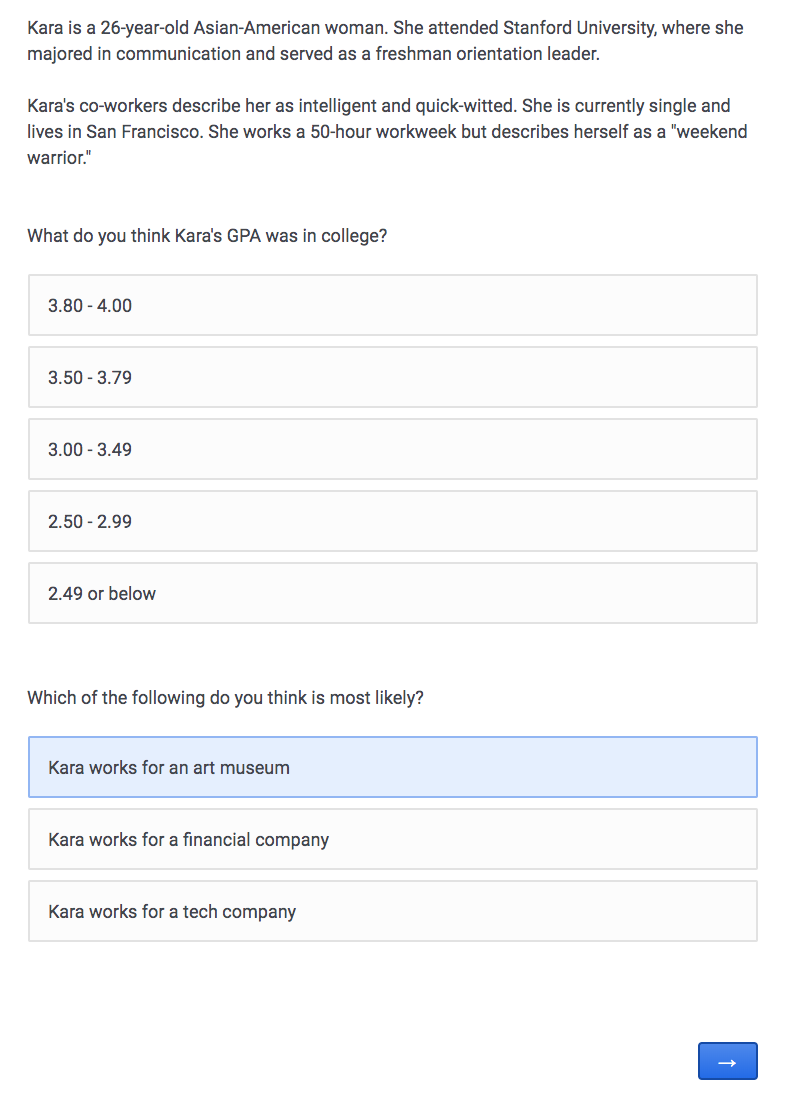
\includegraphics[width=1\textwidth]{../figs/vig_kara.png}
	\caption{}
\end{subfigure}
\begin{subfigure}[t]{0.48\textwidth}
	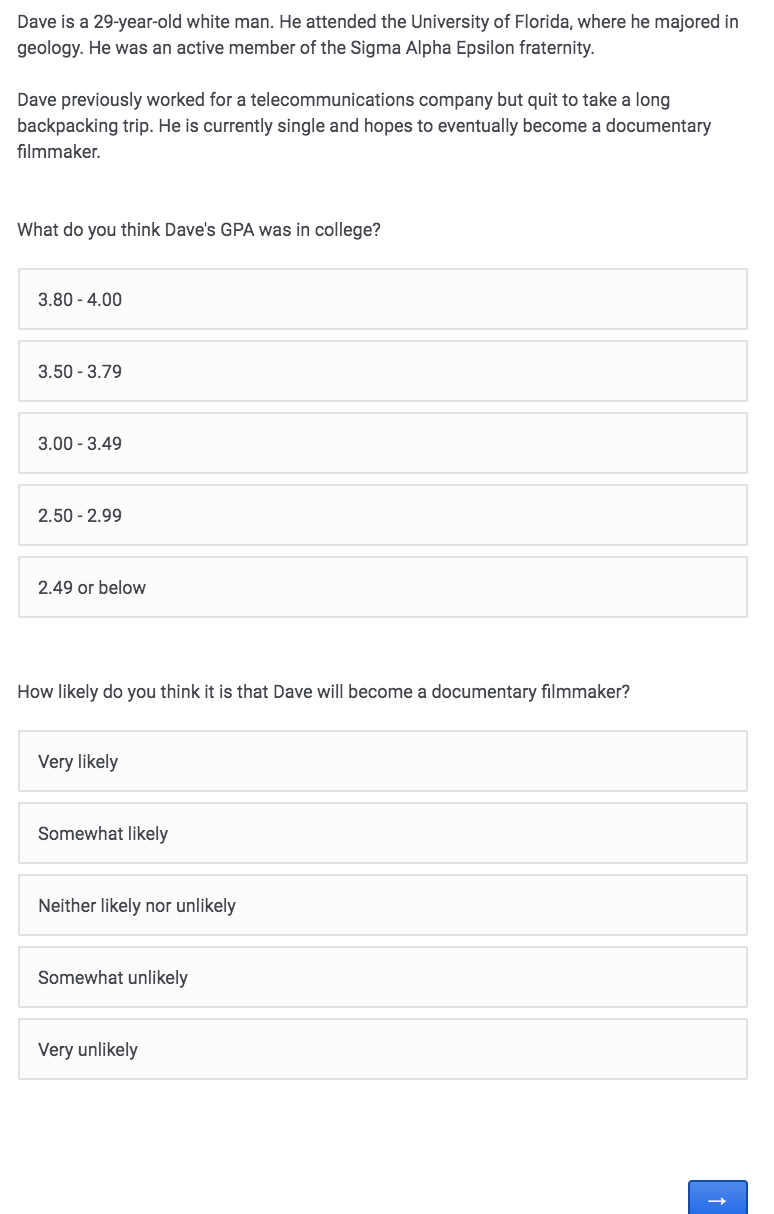
\includegraphics[width=1\textwidth]{../figs/vig_dave.png}
	\caption{}
\end{subfigure}
\end{figure}

\begin{figure}[h!]
\centering
\caption{Vignettes for our modified Linda Problem and the maximal-contrast James experiment}\label{ep_figure_si}
\vspace{5mm}
\begin{subfigure}[t]{0.48\textwidth}
	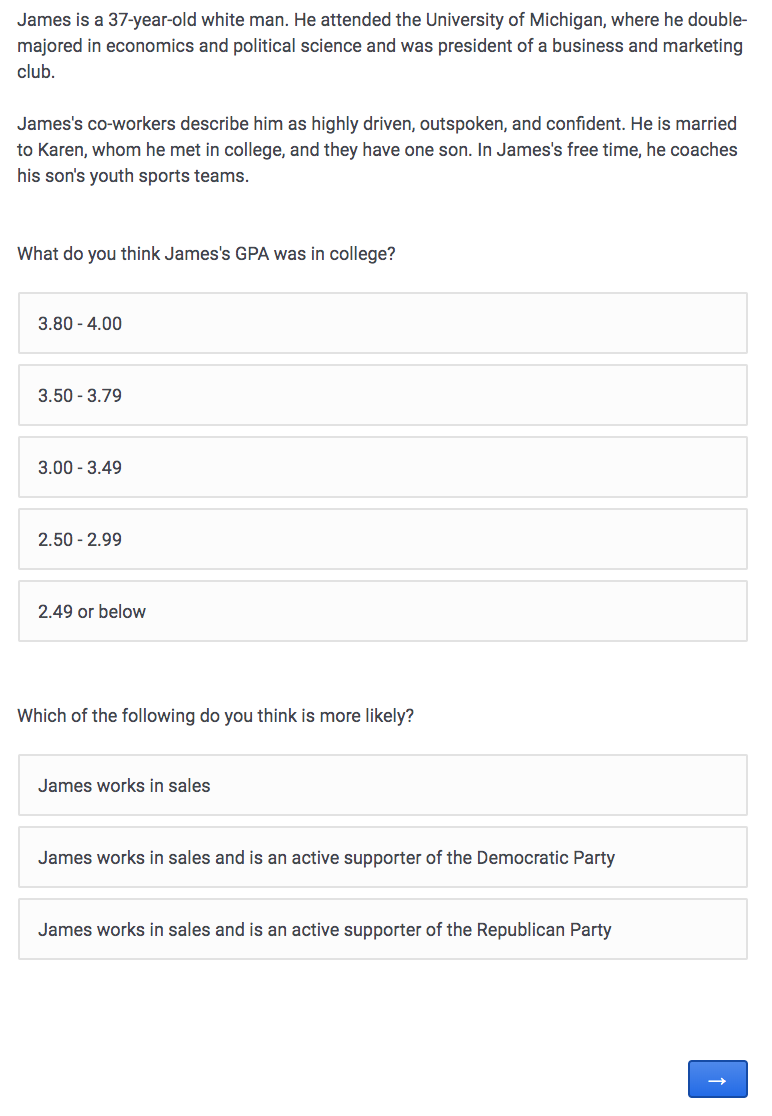
\includegraphics[width=1\textwidth]{../figs/vig_james.png}
	\caption{}
\end{subfigure}
\begin{subfigure}[t]{0.48\textwidth}
	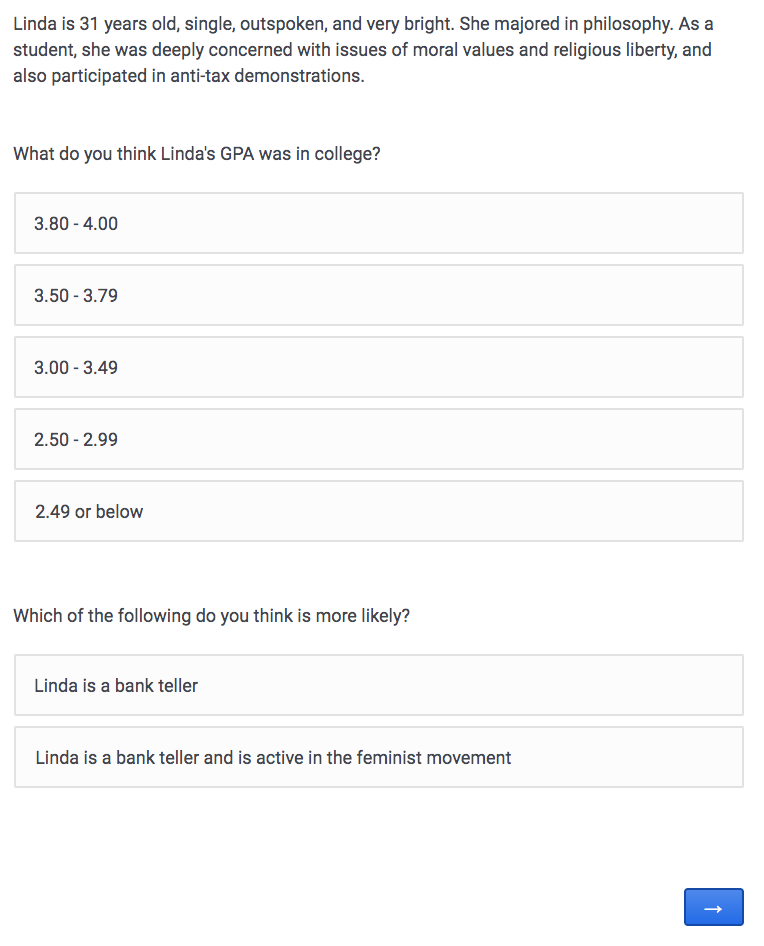
\includegraphics[width=1\textwidth]{../figs/vig_linda.png}
	\caption{}
\end{subfigure}
\end{figure}

\clearpage

\subsection{Bayesian Perceptions}

\subsubsection{Recall battery for treatment impact}
\begin{figure}[h!]
\begin{center}
\caption{Recall Treatment} \label{si_treat_fig}
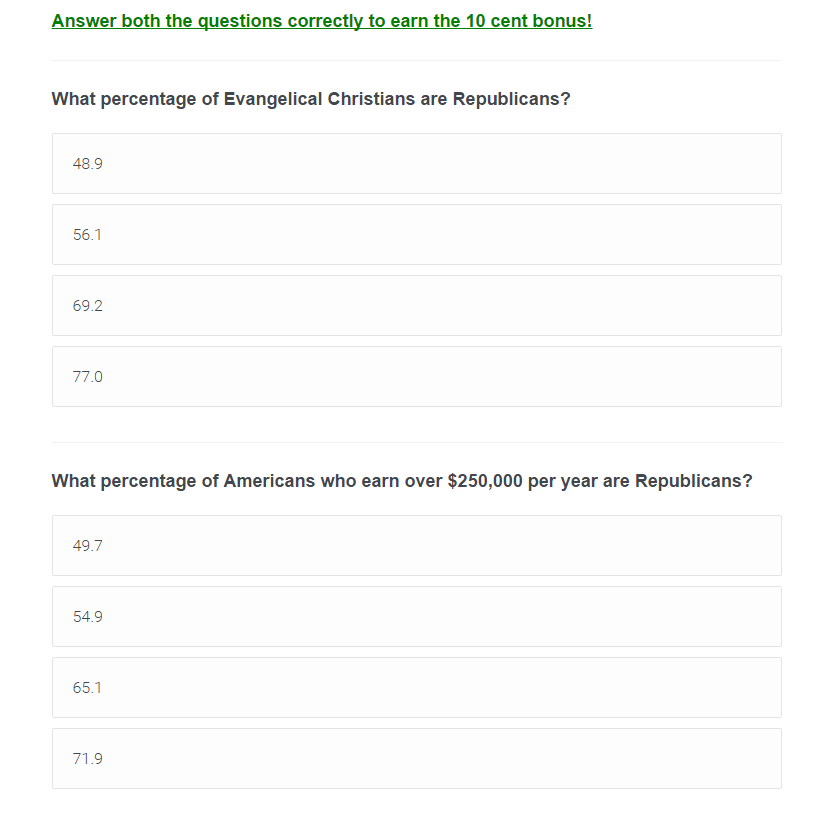
\includegraphics[scale=0.5]{../figs/correct_bonus.png}
\end{center}
\end{figure}

\clearpage
\subsubsection{Numeracy Battery}
\label{oa:num_battery}

The four items used for a numeracy battery are drawn from \citet{weller2012development}. They are:

\begin{enumerate}
\item ``Someone rolls a fair, six-sided die 1,000 times. On average, how many times would the die come up as an even number?'' (Open-ended text-entry response)

\item ``There is a 1\% chance of winning a \$10 prize in the Megabucks Lottery. On average, how many people would win the \$10 prize if 1,000 people each bought a single ticket?'' (Open-ended text-entry response)

\item ``Which of the following numbers represents a bigger risk of getting a disease?'' 
    \begin{itemize}
    \item 1 in 12
    \item 1 in 37
    \end{itemize}
    
\item ``In the PCH Sweepstakes, the chances of winning a car are 1 in 1,000. What percent of PCH Sweepstakes tickets win a car?'' (Open-ended text-entry response)
\end{enumerate}

\clearpage

\section{Filtering protocol for the fully-factorial ``James'' experiment} \label{si:filtering}

At the time we fielded the second ``James'' study, a panic had broken out among experimental social scientists regarding data quality on Mechanical Turk \citep[e.g.,][]{ahler2019turk_nyu, bai_2018, ryan_2018}. In particular, concerns about bot respondents, foreign respondents, and ``account farms'' (locations with multiple individuals taking the same survey, or one individual with multiple accounts) masquerading as genuine survey-takers. We implemented a filtering protocol consistent with \citep{ahler2019turk_nyu} to preclude these concerns. We recruited 1,991 respondents for our original sample. Using \citet{kyip}, we discovered 359 IP addresses flagged for being outside the United States or on a known Blacklist, and an additional 106 duplicated addresses and 9 missing addresses. We classified these as suspicious responses. 87 respondents were also flagged for responding to multiple low-incidence screener questions used to identify potential survey ``trolls'' \citep{lopezhillygus_2018}. In all---there was some overlap between the IP flags and the low-incidence screener flags---we found 484 respondents (24\% of the sample) to be potentially low-quality, leaving us with our final sample of $n =$ 1,507. 

Although the suspicious respondents add noise to the data, they do not change our findings, either in terms of statistical or substantive significance. All of the treatments significantly affect perceptions of James---and the likelihood of committing the conjunction fallacy---as they do in the analysis limited to non-suspicious respondents. Furthermore, the cues about James's race and sexuality continue to be the strongest treatments.

\clearpage

\section{Model results: Fully-factorial ``James'' experiment} \label{si:james_ff_model}

As described in the paper, for the fully-factorial ``James'' experiment our model takes the following form, with $i$ indexing respondents and $j$ indexing possible values of the dependent variable:

\begin{equation}
p_{ij} = p(y_{i} = j) =
    \begin{cases}
p(y_{i} = -1) = p(y_{i}^{*} \leq \alpha_{-1}) \\
p(y_{i} = 0) = p(\alpha_{-1} < y_{i}^{*} \leq \alpha_{0}) \\
p(y_{i} = 1) = p(\alpha_{0} < y_{i}^{*})
    \end{cases}
\end{equation}

\noindent where $y^{*}_{i}$ is the respondent's latent outcome and $\alpha_{-1}$ and $\alpha_{0}$ are the model's cutpoints. We model these probabilities as follows:

\begin{equation}
p(y_{i} = j) \sim \text{logit}^{-1}(\beta_{k}X_{ik} + \varepsilon_{i})
\end{equation}

\noindent where $X_{k}$ denotes our treatment vector---James's race, sexual orientation, religion, and policy views. Importantly, $\beta_{k}$ captures the effect of attribute attribute $k$, averaged over all other attributes in $K$. 

The results of the model are presented in Table \ref{tab:logit_james}. The coefficients, converted to changes in predicted probability of making the Democratic and Republican conjunction fallacies (depicted in Figure 3, are subsequently presented in Table \ref{tab:logit_james_pp}.


% Table created by stargazer v.5.2.2 by Marek Hlavac, Harvard University. E-mail: hlavac at fas.harvard.edu
% Date and time: Sat, Jan 22, 2022 - 5:21:32 PM
\begin{table}[!htbp] \centering 
  \caption{Full model results for the fully-factorial ``James'' experiment} 
  \label{tab:logit_james} 
\begin{tabular}{@{\extracolsep{5pt}}lc} 
\\[-1.8ex]\hline \\[-1.8ex] 
\\[-1.8ex] & \textbf{\shortstack{DV: Democratic (+1) \\ or Republican (-1) conjunction fallacy}} \\ 
\hline \\[-1.8ex] 
 Black (vs. white) & $-$0.61$^{***}$ \\ 
  & (0.10) \\ 
  Gay (vs. straight) & $-$0.82$^{***}$ \\ 
  & (0.10) \\ 
  Evangelical (vs. nothing) & 0.26$^{**}$ \\ 
  & (0.12) \\ 
  Secular (vs. nothing) & $-$0.29$^{**}$ \\ 
  & (0.13) \\ 
  Liberal (vs. nothing) & $-$0.41$^{***}$ \\ 
  & (0.13) \\ 
  Conservative (vs. nothing) & 0.36$^{***}$ \\ 
  & (0.12) \\ 
 N & 1507 \\ 
\hline \\[-1.8ex] 
\multicolumn{2}{l}{$^{***}$p $<$ .01; $^{**}$p $<$ .05; $^{*}$p $<$ .1} \\ 
\end{tabular} 
\end{table} 

% latex table generated in R 4.1.2 by xtable 1.8-4 package
% Sun Jan 30 17:15:54 2022
\begin{table}[!htb]
\centering
\caption{Model coefficients converted to changes in predicted probabilities in the fully-factorial ``James'' experiment} 
\label{tab:logit_james_pp}
\begingroup\small
\begin{tabular}{lccc}
  \hline
When James is described as & Effect & Lower CI & Upper CI \\ 
  \hline
Black (vs. white) Dem-CF & 15.00 & 10.10 & 19.90 \\ 
  Black (vs. white) Rep-CF & -9.70 & -12.84 & -6.56 \\ 
  Conservative (vs. no cue) Dem-CF & -9.00 & -15.08 & -2.92 \\ 
  Conservative (vs. no cue) Rep-CF & 6.00 & 1.88 & 10.12 \\ 
  Evangelical (vs. no cue) Dem-CF & -6.40 & -12.28 & -0.52 \\ 
  Evangelical (vs. no cue) Rep-CF & 4.20 & 0.28 & 8.12 \\ 
  Gay (vs. straight) Dem-CF & 20.10 & 15.20 & 25.00 \\ 
  Gay (vs. straight) Rep-CF & -13.20 & -16.53 & -9.87 \\ 
  Liberal (vs. no cue) Dem-CF & 10.10 & 4.22 & 15.98 \\ 
  Liberal (vs. no cue) Rep-CF & -6.40 & -10.12 & -2.68 \\ 
  Secular (vs. no cue) Dem-CF & 7.10 & 1.02 & 13.18 \\ 
  Secular (vs. no cue) Rep-CF & -4.50 & -8.22 & -0.78 \\ 
   \hline
\end{tabular}
\endgroup
\end{table}


\clearpage
\subsection{Marginals for the James experiment: How often do respondents make the conjunction fallacy?} \label{si:marginals}

An alternative way to present these results is simply to show how often respondents commit the conjunction fallacies when presented with party-representative traits of James. This is shown in the table below (see Table \ref{tab:james_marginal}), which also implies why changes in predicted probabilities are a better way to assess the effects of this information. For reasons not entirely clear, respondents were far more likely to commit the Democratic conjunction fallacy---that is, to say that James is X and a Democrat---than to commit the equivalent Republican conjunction fallacy, sometimes even for counter-representative groups. (For example, when James is given a conservative cue, respondents are still more likely to commit the Democratic conjunction fallacy. However, the rate at which people commit the Republican conjunction fallacy goes up when James is described as conservative, and is in between these two quantities when James lacks an ideological cue.) We suspect that the Democratic conjunction fallacy is more popular for several reasons but, first and foremost, that James is described as college educated at a time when a serious degree divide has opened up between the two parties. Additionally, if anything, respondents appear ever so slightly more likely to attribute their own partisanship to James, all else equal.

One interesting thing that stands out is that Democrats and Republicans commit the conjunction fallacy at higher rates than independents, even when the rates they commit these errors are quite similar to each other---even when assessing the other party. This is relatively consistent with the results in Ahler \& Sood (2018): everyone stereotypes, but partisans are more prone to do so than independents.

% latex table generated in R 4.1.2 by xtable 1.8-4 package
% Sun Jan 30 17:15:56 2022
\begin{table}[!htb]
\centering
\caption{Marginal rates at which conjunction fallacies (CFs) are committed, given particular traits of ``James''} 
\label{tab:james_marginal}
\begingroup\small
\begin{tabular}{lcccc}
  \hline
Group-CF dyad & Full sample & Democrats & Independents & Republicans \\ 
  \hline
Black-Dem. CF & 0.60 & 0.66 & 0.49 & 0.54 \\ 
  Black-Rep. CF & 0.15 & 0.12 & 0.10 & 0.21 \\ 
  White-Dem. CF & 0.49 & 0.50 & 0.38 & 0.49 \\ 
  White-Rep. CF & 0.28 & 0.28 & 0.20 & 0.29 \\ 
  Gay-Dem. CF & 0.63 & 0.68 & 0.48 & 0.60 \\ 
  Gay-Rep. CF & 0.14 & 0.12 & 0.08 & 0.19 \\ 
  Straight-Dem. CF & 0.46 & 0.49 & 0.38 & 0.44 \\ 
  Straight-Rep. CF & 0.29 & 0.29 & 0.25 & 0.31 \\ 
  Evangelical-Dem. CF & 0.49 & 0.52 & 0.38 & 0.48 \\ 
  Evangelical-Rep. CF & 0.27 & 0.25 & 0.25 & 0.29 \\ 
  Secular-Dem. CF & 0.61 & 0.67 & 0.48 & 0.55 \\ 
  Secular-Rep. CF & 0.16 & 0.16 & 0.12 & 0.18 \\ 
  No relig. cue-Dem. CF & 0.54 & 0.56 & 0.45 & 0.52 \\ 
  No relig. cue-Rep. CF & 0.21 & 0.20 & 0.08 & 0.27 \\ 
  Liberal-Dem. CF & 0.63 & 0.69 & 0.43 & 0.60 \\ 
  Liberal-Rep. CF & 0.15 & 0.13 & 0.15 & 0.17 \\ 
  Conserv.-Dem. CF & 0.47 & 0.49 & 0.35 & 0.46 \\ 
  Conserv.-Rep. CF & 0.29 & 0.29 & 0.15 & 0.33 \\ 
  No ideo cue-Dem. CF & 0.53 & 0.55 & 0.54 & 0.49 \\ 
  No ideo cue-Rep. CF & 0.21 & 0.19 & 0.16 & 0.26 \\ 
   \hline
\end{tabular}
\endgroup
\end{table}


\clearpage
\subsection{Results From the Full Interaction Model}
If the estimand of interest is the main treatment effect and not AMCE, which is the composite treatment effect, a weighted-average of the interactions with other treatments, then we need to estimate a full interaction model, which we do below (see Table ~\ref{tab:logit_james_interaction}). As the results show, the main effect of changing race of James to black (vs. white), his sexual orientation to gay (vs. heterosexual), changing his ideological position to liberal (vs. offering no cue), and making him secular (vs. offering no cue), all have large significants in the expected direction. However, the main effects for changing religious affiliation to Evangelical (vs. no cue) and changing ideological position to Conservative (vs. no clue) are small and statistically insignificant (unlike results in Table \ref{tab:logit_james}).


% Table created by stargazer v.5.2.2 by Marek Hlavac, Harvard University. E-mail: hlavac at fas.harvard.edu
% Date and time: Sun, Jan 30, 2022 - 5:15:36 PM
\begin{table}[!htbp] \centering 
  \caption{Full interaction model results for the fully-factorial ``James'' experiment} 
  \label{tab:logit_james_interaction} 
\tiny 
\begin{tabular}{@{\extracolsep{5pt}}lc} 
\\[-1.8ex]\hline \\[-1.8ex] 
\\[-1.8ex] & \textbf{\shortstack{DV: Democratic (+1) \\ or Republican (-1) conjunction fallacy}} \\ 
\hline \\[-1.8ex] 
 Black (vs. white) & $-$1.32$^{***}$ \\ 
  & (0.41) \\ 
  Gay (vs. straight) & $-$1.17$^{***}$ \\ 
  & (0.40) \\ 
  Evangelical (vs. nothing) & 0.13 \\ 
  & (0.39) \\ 
  Secular (vs. nothing) & $-$0.75$^{*}$ \\ 
  & (0.41) \\ 
  Liberal (vs. nothing) & $-$1.39$^{***}$ \\ 
  & (0.42) \\ 
  Conservative (vs. nothing) & $-$0.11 \\ 
  & (0.45) \\ 
  Black * Gay & 0.24 \\ 
  & (0.65) \\ 
  Black * Evangelical & 0.13 \\ 
  & (0.57) \\ 
  Gay * Evangelical & $-$0.39 \\ 
  & (0.57) \\ 
  Black* Secular & 0.52 \\ 
  & (0.61) \\ 
  Gay * Secular & 0.04 \\ 
  & (0.61) \\ 
  Black * Liberal & 1.26$^{**}$ \\ 
  & (0.58) \\ 
  Gay *Liberal & 0.56 \\ 
  & (0.60) \\ 
  Evangelical * Liberal & 1.35$^{**}$ \\ 
  & (0.58) \\ 
  Secular * Liberal & 1.01$^{*}$ \\ 
  & (0.60) \\ 
  Black * Conservative & 0.71 \\ 
  & (0.62) \\ 
  Gay * Conservative & 0.57 \\ 
  & (0.59) \\ 
  Evangelical * Conservative & 0.27 \\ 
  & (0.59) \\ 
  Secular * Conservative & 0.66 \\ 
  & (0.64) \\ 
  Black * Gay * Evangelical & 0.86 \\ 
  & (0.88) \\ 
  Black * Gay * Secular & 0.58 \\ 
  & (0.92) \\ 
  Black * Gay * Liberal & $-$0.46 \\ 
  & (0.92) \\ 
  Black * Evangelical * Liberal & $-$1.78$^{**}$ \\ 
  & (0.82) \\ 
  Gay * Evangelical * Liberal & $-$0.44 \\ 
  & (0.84) \\ 
  Black * Secular * Liberal & $-$1.12 \\ 
  & (0.86) \\ 
  Gay * Secular * Liberal & $-$0.67 \\ 
  & (0.88) \\ 
  Black * Gay * Conservative & $-$0.15 \\ 
  & (0.89) \\ 
  Black * Evangelical * Conservative & $-$0.39 \\ 
  & (0.83) \\ 
  Gay * Evangelical  * Conservative & $-$0.30 \\ 
  & (0.85) \\ 
  Black * Secular * Conservative & $-$0.92 \\ 
  & (0.89) \\ 
  Gay * Secular * Conservative & $-$0.95 \\ 
  & (0.87) \\ 
  Black * Gay * Evangelical * Liberal & 0.44 \\ 
  & (1.25) \\ 
  Black * Gay * Secular * Liberal & 1.14 \\ 
  & (1.30) \\ 
  Black * Gary * Evangelical * Conservative & $-$0.39 \\ 
  & (1.22) \\ 
  Black * Gay * Secular * Conservative & 0.61 \\ 
  & (1.27) \\ 
 N & 1507 \\ 
\hline \\[-1.8ex] 
\multicolumn{2}{l}{$^{***}$p $<$ .01; $^{**}$p $<$ .05; $^{*}$p $<$ .1} \\ 
\end{tabular} 
\end{table} 


\section{The Ubiquity of Party Stereotypes?}

But even when people are encouraged to process slowly and deliberately, their party stereotypes still yield cognitive bias. In August 2018, we conducted an experiment showing just this. We presented 138 research participants from Amazon's Mechanical Turk with the image in Figure \ref{fig:avatar_shown}, requiring them to stay on that screen for 15 seconds before they could advance the survey. Figure \ref{fig:avatar_shown} presents two groups of 25 avatars, one side in blue shirts and the other in red. The avatars differ in race, gender, and general appearance but, importantly, both ``parties'' contain the exact same 25 images. (We randomized both which side was the ``Democratic'' side and the order of avatars in the figure.) After advancing the screen, participants indicated the number of ``people'' in each party they saw who were: men or women, and Black, white, or another race/ethnicity, with a counter tool provided to help with summation to 25. 

\begin{figure}[p!] 
\centering
\caption{People are given identical images but report systematically different beliefs about what they saw}\label{fig:avatars}
\vspace{10mm}
\begin{subfigure}[t]{1\textwidth}
	\caption{What respondents saw}
	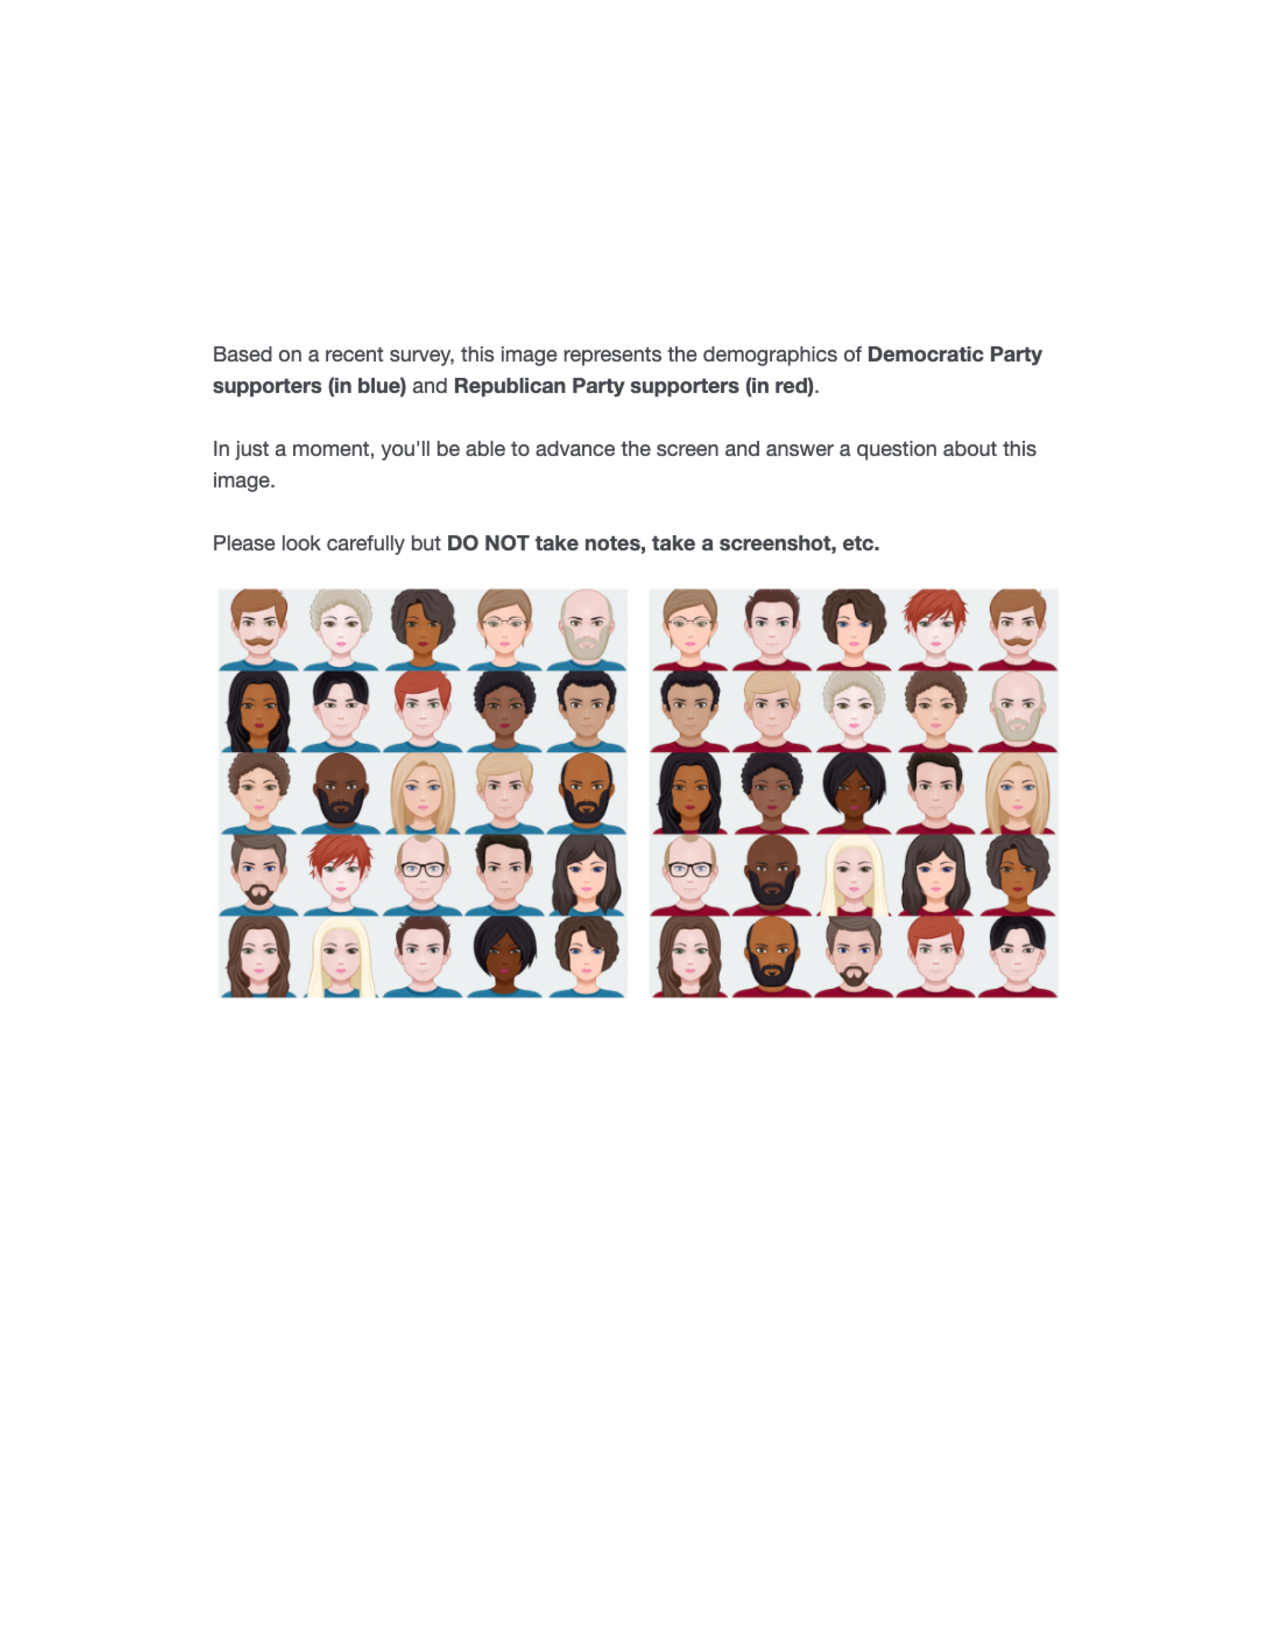
\includegraphics[width=1\textwidth]{../figs/avatar_exp.pdf} \label{fig:avatar_shown}
\end{subfigure}
\end{figure}
\begin{figure}
\ContinuedFloat
\begin{subfigure}[t]{1\textwidth}
	\caption{What respondents reported}
	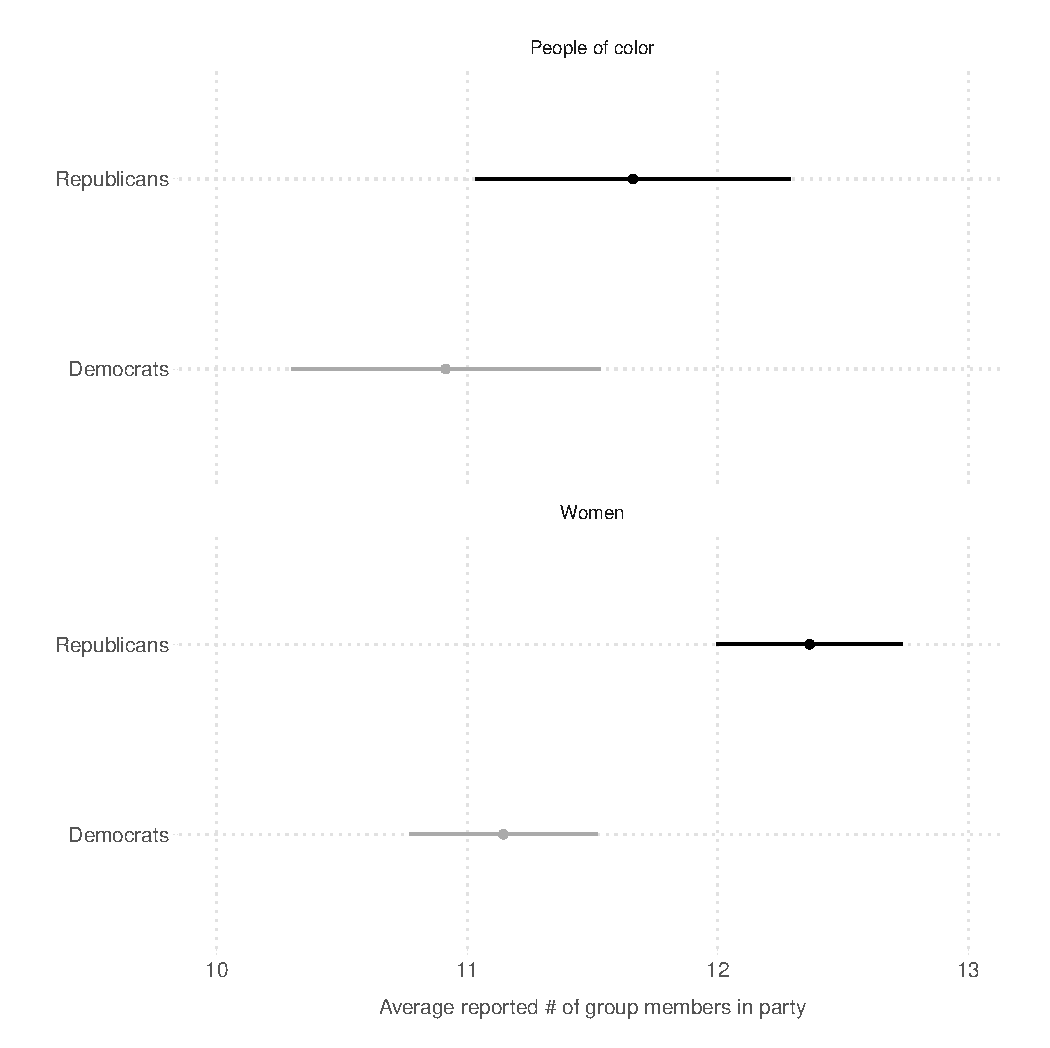
\includegraphics[width=1\textwidth]{../figs/fig_si_41_avatars.pdf} \label{fig:avatar_guessed}
\end{subfigure}
\end{figure}

If people's party stereotypes are not central to how they process political information, then we would expect participants to report equal numbers of women and non-white avatars on each side of the image in Figure \ref{fig:avatar_shown}. Despite our alerting participants to having to answer questions about the images and requiring them to spend time on that screen, only 26.4\% correctly identified the same number of women across images and just 25.8\% correctly reported equal numbers of non-white avatars on both sides. On average, as Figure \ref{fig:avatar_guessed} shows, participants identified 1.2 more women and 0.8 more people of color wearing blue shirts than red shirts. Although we provided identical images and encouraged more thoughtful processing, respondents still erred systematically, and consistent with party stereotypes, while reporting what they saw.\footnote{One implication that might be tested in future work is whether respondents would perform better at this admittedly tough task if they were presented two sides separated by race or gender, with shirt color varying within each side. This would allow researchers to assess how effectively people can recognize $p($party $|$ group$)$, the quantity that is more often presented in news and polling reports and which we argue contributes to the use of representativeness heuristics.}

When most people process political information, they tend to do so haphazardly and automatically \citep{citrin1990self, lodge2013rationalizing, Sears1983, westen2006neural}---not in carefully controlled information environments guiding their processing, and usually handling more (and more complex) information than what we can convey with 50 avatars. Thus, we suspect that party stereotyping is not only an automatic process, but also a foremost reasoning device.% for people as they navigate the political environment.

\clearpage

\bibliographystyle{apsr}
\bibliography{typecast.bib}

\end{document}

